\documentclass[10pt]{article}
\usepackage[a4paper,margin=18mm]{geometry}
\usepackage[T1]{fontenc}\usepackage{lmodern}
\usepackage{amsmath,amssymb,booktabs,array,enumitem}
\usepackage{tikz}\usetikzlibrary{shapes.gates.logic.US,positioning,arrows.meta}
\usepackage[hidelinks]{hyperref}
\setlength{\parindent}{0pt}\setlength{\parskip}{4pt}\setlength{\emergencystretch}{2em}
\newcommand{\mos}[4]{\begin{scope}[shift={(#1,#2)}]
\draw(0,.24)--(0,-.24);\draw(0,.2)--(.25,.2)--(.25,.5);\draw(0,-.2)--(.25,-.2)--(.25,-.5);
\draw(-.16,.23)--(-.16,-.23);
\ifnum#4=1\draw(-.26,0)circle(.06);\draw(-.75,0)--(-.32,0);\else\draw(-.75,0)--(-.16,0);\fi
\node[anchor=east,font=\scriptsize]at(-.76,0){$#3$};\end{scope}}
\newcommand{\gnd}[2]{\draw(#1,#2)--(#1,{#2-.12});\draw({#1-.17},{#2-.12})--({#1+.17},{#2-.12});\draw({#1-.11},{#2-.2})--({#1+.11},{#2-.2});}
\newcommand{\rail}[3]{\draw(#1,#2)--(#1,{#2+.14});\node[above,font=\scriptsize]at(#1,{#2+.14}){$#3$};}
\begin{document}
\begin{center}{\Large EE3032 Introduction to VLSI Design---Final}\\Fall 2008\end{center}
Reconstructed from the complete three-page scanned original, printed pages 1-1 through 1-3. Question weights total \textbf{115\%}. The original Fall 2008 footer controls the year; handwritten annotations are not transcribed as prompt text. All source circuit polarities, full function overbar and sizing labels are retained in editable TikZ. The reconstruction preserves the printed mathematical premises.\par\medskip
\textbf{1. (30\%)} Answer the following problems.
\begin{enumerate}[label=(\alph*)]
\item List two methods for reducing the power bounce and ground bounce in the IO pads. (4\%)
\item List major steps of the CMOS full-custom design flow. (6\%)
\item List two methods for reducing the switching power of a CMOS circuit. (4\%)
\item Explain the energy consumption of an inverter when the inverter performs a switching. (4\%)
\item List two major problems of dynamic logic. (4\%)
\item List two limitations of CMOS domino logic. (4\%)
\item What are core-limited design and pad-limited design? (4\%)
\end{enumerate}\textbf{2. (15\%)} Sketch the Boolean function $f=\overline{A(B+C)+DE}$ using each of the following circuit techniques. (1) Domino logic (5\%) (2) Fully differential logic (5\%) (3) Static CMOS logic (5\%).\par\medskip\textbf{3. (10\%)} Explain the operation principle of the circuit shown in Figure 1.\begin{center}\begin{tikzpicture}[scale=.9,font=\small]
\foreach \x in {0,3,6,9}{\rail{\x+.25}{4}{V_{DD}}\gnd{\x+.25}{.2}}
\mos{0}{3.5}{}{1}\mos{0}{2.1}{\phi}{1}\mos{0}{.7}{}{0}\draw(.25,3)--(.25,2.6);\draw(.25,1.6)--(.25,1.2);
\mos{3}{3.5}{}{1}\mos{3}{2.1}{\phi}{1}\mos{3}{.7}{}{0}\draw(3.25,3)--(3.25,2.6);\draw(3.25,1.6)--(3.25,1.2);
\mos{6}{3.5}{}{1}\mos{6}{2.1}{\phi}{0}\mos{6}{.7}{}{0}\draw(6.25,3)--(6.25,2.6);\draw(6.25,1.6)--(6.25,1.2);
\mos{9}{3.5}{}{1}\mos{9}{2.1}{\phi}{0}\mos{9}{.7}{}{0}\draw(9.25,3)--(9.25,2.6);\draw(9.25,1.6)--(9.25,1.2);
\draw(-.75,3.5)--(-1.3,3.5)--(-1.3,.7)--(-.75,.7);\draw(-1.3,2.8)--(-2,2.8)node[left]{$I$};\draw(.25,1.4)--(1.7,1.4)--(1.7,3.5)--(2.25,3.5);\draw(1.7,1.4)--(1.7,.7)--(2.25,.7);\node[above]at(.8,1.4){$A$};\fill(1.7,1.4)circle(1.5pt);
\draw(3.25,1.4)--(4.7,1.4)--(4.7,3.5)--(5.25,3.5);\draw(4.7,1.4)--(4.7,.7)--(5.25,.7);\node[above]at(3.9,1.4){$B$};\fill(4.7,1.4)circle(1.5pt);
\draw(6.25,2.8)--(7.7,2.8)--(7.7,3.5)--(8.25,3.5);\draw(7.7,2.8)--(7.7,.7)--(8.25,.7);\node[below]at(6.9,2.8){$C$};\fill(7.7,2.8)circle(1.5pt);\draw(9.25,2.8)--(11,2.8)node[right]{$O$};
\end{tikzpicture}\\Figure 1: A dynamic CMOS register circuit. All four three-device stages and the two first-stage clock-controlled pMOS bubbles are retained.\end{center}\newpage\textbf{4. (15\%)} The circuit shown in Figure 2 results from the implementation of a high-speed one-bit full adder. Complete the following problems.
\begin{enumerate}[label=(\alph*)]
\item What type of CMOS logic style is used to implement this circuit? (5\%)
\item Suppose that the drain capacitance and gate capacitance of the PMOS and NMOS are $0.2\,fF$ and $1\,fF$, respectively. The leakage current of the output nodes $\bar C_{n+1}$ and $\bar S_n$ is $1\,nA$. Also, $V_{dd}=1.8\,V$ and the switching threshold voltage of the inverter is $1\,V$. Determine the lowest speed at which the circuit should be operated. (10\%)
\end{enumerate}\begin{center}\begin{tikzpicture}[scale=.75,font=\small]
\mos{0}{3.6}{\phi}{1}\rail{.25}{4.1}{V_{DD}}\draw(.25,3.1)--(.25,2.6);\draw(-1.75,2.6)--(2.25,2.6);\fill(.25,2.6)circle(1.5pt);\node[above]at(1.2,2.6){$\bar C_{n+1}$};
\mos{-2}{1.8}{A_n}{0}\mos{-2}{.4}{B_n}{0}\draw(-1.75,2.6)--(-1.75,2.3);\draw(-1.75,1.3)--(-1.75,.9);
\mos{1}{1.8}{C_n}{0}\draw(1.25,2.6)--(1.25,2.3);\draw(1.25,1.3)--(1.25,1.1);\draw(.25,1.1)--(2.25,1.1);\mos{0}{.4}{A_n}{0}\mos{2}{.4}{B_n}{0}\draw(.25,1.1)--(.25,.9);\draw(2.25,1.1)--(2.25,.9);
\draw(-1.75,-.1)--(-1.75,-.4)--(2.25,-.4)--(2.25,-.1);\draw(.25,-.1)--(.25,-.8);\fill(.25,-.4)circle(1.5pt);\mos{0}{-1.3}{\phi}{0}\gnd{.25}{-1.8}
\node[not gate US,draw,rotate=-90](ix)at(3.5,1.2){};\draw(2.25,2.6)--(3.5,2.6)--(ix.input);\draw(ix.output)--(3.5,.15)node[below]{$C_{n+1}$};
\mos{8}{3.9}{\bar\phi}{1}\rail{8.25}{4.4}{V_{DD}}\draw(8.25,3.4)--(8.25,3.1);\draw(6.25,3.1)--(10.25,3.1);\mos{6}{2.4}{A_n}{1}\mos{8}{2.4}{B_n}{1}\mos{10}{2.4}{C_n}{1}
\foreach \x in {6.25,8.25,10.25}{\draw(\x,3.1)--(\x,2.9);\draw(\x,1.9)--(\x,1.6);}\draw(6.25,1.6)--(10.25,1.6);
\mos{6}{.7}{}{1}\mos{10}{.7}{A_n}{1}\mos{10}{-.7}{B_n}{1}\mos{10}{-2.1}{C_n}{1}\draw(6.25,1.6)--(6.25,1.2);\draw(10.25,1.6)--(10.25,1.2);\draw(10.25,.2)--(10.25,-.2);\draw(10.25,-1.2)--(10.25,-1.6);
\node[above]at(9,-3){$\bar S_n$};\draw(6.25,.2)--(6.25,-3)--(10.25,-3)--(10.25,-2.6);\draw(8.25,-3)--(8.25,-3.35);\mos{8}{-3.85}{\bar\phi}{0}\gnd{8.25}{-4.35}
\draw(2.25,2.6)--(4.6,2.6)--(4.6,.7)--(5.25,.7);\fill(3.5,2.6)circle(1.5pt);\node[not gate US,draw,rotate=-90](iy)at(11.7,-3.25){};\draw(10.25,-3)--(11.7,-3)--(iy.input);\draw(iy.output)--(11.7,-4.2)node[below]{$S_n$};
\end{tikzpicture}\\Figure 2: An adder circuit. The printed static output inverters are retained.\end{center}\textbf{5. (10\%)} Figure 3 shows a sequential circuit (pipelined circuit). Assume that your boss asks you to design the circuit such that the circuit can be operated at $100\,MHz$. Also, assume that the clock-to-Q propagation delay, the setup time, and the hold time of registers R1 and R2 are $1\,ns$, $1.5\,ns$, and $1\,ns$, respectively. How fast should the combinational circuit be designed?\begin{center}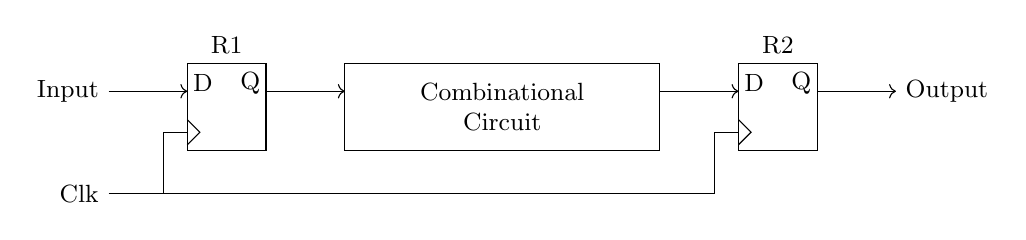
\begin{tikzpicture}[font=\small]
\foreach \x/\name in {0/R1,7/R2}{\draw(\x,-.45)rectangle(\x+1,.65);\node at(\x+.2,.4){D};\node at(\x+.8,.4){Q};\draw(\x,-.38)--(\x+.16,-.22)--(\x,-.06);\node[above]at(\x+.5,.65){\name};\draw(\x-.3,-1)--(\x-.3,-.22)--(\x,-.22);}
\draw(2,.65)rectangle(6,-.45);\node[align=center]at(4,.1){Combinational\\Circuit};\draw[->](-1,.3)--(0,.3);\node[left]at(-1,.3){Input};\draw[->](1,.3)--(2,.3);\draw[->](6,.3)--(7,.3);\draw[->](8,.3)--(9,.3)node[right]{Output};\draw(-1,-1)--(6.7,-1);\node[left]at(-1,-1){Clk};
\end{tikzpicture}\\Figure 3: A pipelined circuit.\end{center}\newpage\textbf{6. (10\%)} Figure 4 shows the Schmitt CMOS circuit and its voltage transfer curve. Assume that the Schmitt circuit is designed as $V_{T+}=0.7V_{dd}$ and $V_{T-}=0.3V_{dd}$. Also, the size of N1 is $(W/L)_{n1}=2\,\mu m/0.5\,\mu m$ and the size of P1 is $(W/L)_{p1}=3\,\mu m/0.5\,\mu m$. What sizes of N3 and P3 should be designed?\begin{center}\begin{tikzpicture}[scale=.91,font=\small]
\mos{0}{3.8}{}{1}\mos{0}{2.4}{}{1}\mos{0}{1}{}{0}\mos{0}{-.4}{}{0}
\rail{.25}{4.3}{V_{dd}}\draw(.25,3.3)--(.25,2.9);\draw(.25,1.9)--(.25,1.5);\draw(.25,.5)--(.25,.1);\gnd{.25}{-.9}
\draw(-.75,3.8)--(-1.25,3.8)--(-1.25,-.4)--(-.75,-.4);\draw(-1.25,2.4)--(-.75,2.4);\draw(-1.25,1)--(-.75,1);\draw(-1.25,1.7)--(-1.8,1.7)node[left]{$V_{in}$};
\node[right]at(.4,3.8){P1};\node[right]at(.4,2.4){P2};\node[right]at(.4,1){N2};\node[right]at(.4,-.4){N1};
\draw(.25,3.1)--(1.15,3.1);\begin{scope}[shift={(1.65,2.85)},rotate=90]\mos{0}{0}{}{1}\end{scope}\draw(2.15,3.1)--(2.5,3.1);\gnd{2.5}{3.1}\node[above]at(1.6,3.28){P3};
\draw(.25,.3)--(1.15,.3);\begin{scope}[shift={(1.65,.55)},rotate=-90]\mos{0}{0}{}{0}\end{scope}\draw(2.15,.3)--(2.5,.3);\rail{2.5}{.3}{V_{dd}}\node[below]at(1.6,-.2){N3};
\draw(.25,1.7)--(3.3,1.7)node[right]{$V_{out}$};\fill(.25,1.7)circle(1.5pt);\draw(1.65,2.1)--(1.65,1.3);\fill(1.65,1.7)circle(1.5pt);
\begin{scope}[xshift=5.5cm]
\draw[->](0,0)--(4.4,0)node[right]{$V_{in}$};\draw[->](0,0)--(0,3.7)node[above]{$V_{out}$};\node[left]at(0,3){$V_{dd}$};
\draw[thick](0,3)--(2.2,3)..controls(2.75,3)and(2.9,2.4)..(2.9,1.4)..controls(2.9,.3)and(3.4,0)..(4,0);
\draw[thick](0,3)--(.5,3)..controls(1.2,3)and(1.4,2.5)..(1.4,1.4)..controls(1.4,.3)and(2.1,0)..(4,0);
\draw[dashed](1.4,0)--(1.4,1.4);\draw[dashed](2.9,0)--(2.9,1.4);\draw[->](1.85,3)--(2.2,3);\draw[->](2.9,2)--(2.9,1.5);\draw[->](1.4,1.5)--(1.4,2);\draw[->](2.2,0)--(1.85,0);
\node[below]at(1.4,0){$V_{T-}$};\node[below]at(2.9,0){$V_{T+}$};\node[below]at(4,0){$V_{dd}$};\node at(1.8,-.9){(b)};\end{scope}\node at(.7,-1.55){(a)};
\end{tikzpicture}\\Figure 4: (a) A CMOS Schmitt circuit. (b) Its voltage transfer curve.\end{center}\textbf{7. (10\%)} Figure 5 shows the symbolic layouts. Draw the schematic diagrams of the layouts.\begin{center}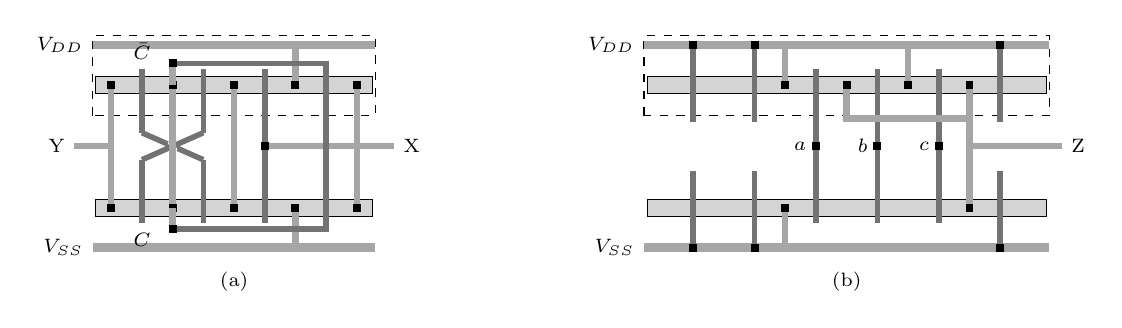
\begin{tikzpicture}[x=.78cm,y=.78cm,font=\scriptsize]
\draw[dashed](-.3,.5)rectangle(4.3,1.8);\foreach \y in {1,-1}{\fill[black!17](-.25,\y-.14)rectangle(4.25,\y+.14);\draw(-.25,\y-.14)rectangle(4.25,\y+.14);}
\foreach \y in {1.65,-1.65}{\draw[line width=3pt,black!35](-.3,\y)--(4.3,\y);}
\node[left]at(-.3,1.65){$V_{DD}$};\node[left]at(-.3,-1.65){$V_{SS}$};
\foreach \x in {.5,1.5}{\draw[line width=2pt,black!55](\x,1.25)--(\x,.22) (\x,-.22)--(\x,-1.25);}
\draw[line width=2pt,black!55](.5,.22)--(1.5,-.22) (.5,-.22)--(1.5,.22);\draw[white,line width=4pt](.96,-.02)--(1.04,.02);\draw[line width=2pt,black!55](.96,-.02)--(1.04,.02);
\node[above]at(.5,1.25){$\bar C$};\node[below]at(.5,-1.25){$C$};
\foreach \x in {2.5,3.5}{\draw[line width=2pt,black!55](\x,-1.25)--(\x,1.25);}
\foreach \x in {0,1,2,4}{\draw[line width=2.3pt,black!35](\x,1)--(\x,-1);\foreach \y in {1,-1}{\fill(\x-.065,\y-.065)rectangle(\x+.065,\y+.065);}}
\draw[line width=2.3pt,black!35](-.6,0)--(0,0) (4,0)--(4.6,0) (2.5,0)--(4,0);
\fill(2.5-.065,-.065)rectangle(2.5+.065,.065);\node[left]at(-.6,0){Y};\node[right]at(4.6,0){X};
\draw[line width=2.3pt,black!35](3,1)--(3,1.65) (3,-1)--(3,-1.65);\foreach \y in {1,-1}{\fill(2.935,\y-.065)rectangle(3.065,\y+.065);}
\draw[line width=2pt,black!55](1,1.35)--(3.5,1.35)--(3.5,-1.35)--(1,-1.35);\draw[line width=2.3pt,black!35](1,1)--(1,1.35) (1,-1)--(1,-1.35);\foreach \y in {1.35,-1.35}{\fill(.935,\y-.065)rectangle(1.065,\y+.065);}
\node at(2,-2.2){(a)};
\begin{scope}[xshift=7cm]
\draw[dashed](-.3,.5)rectangle(6.3,1.8);\foreach \y in {1,-1}{\fill[black!17](-.25,\y-.14)rectangle(6.25,\y+.14);\draw(-.25,\y-.14)rectangle(6.25,\y+.14);}
\foreach \y in {1.65,-1.65}{\draw[line width=3pt,black!35](-.3,\y)--(6.3,\y);}\node[left]at(-.3,1.65){$V_{DD}$};\node[left]at(-.3,-1.65){$V_{SS}$};
\foreach \x in {.5,1.5,5.5}{\draw[line width=2pt,black!55](\x,.4)--(\x,1.65) (\x,-.4)--(\x,-1.65);\foreach \y in {1.65,-1.65}{\fill(\x-.065,\y-.065)rectangle(\x+.065,\y+.065);}}
\foreach \x/\g in {2.5/a,3.5/b,4.5/c}{\draw[line width=2pt,black!55](\x,-1.25)--(\x,1.25);\fill(\x-.065,-.065)rectangle(\x+.065,.065);\node[left]at(\x,0){$\g$};}
\draw[line width=2.3pt,black!35](2,1)--(2,1.65) (4,1)--(4,1.65) (2,-1)--(2,-1.65);\foreach \x in {2,4}{\fill(\x-.065,.935)rectangle(\x+.065,1.065);}\fill(1.935,-1.065)rectangle(2.065,-.935);
\draw[line width=2.3pt,black!35](3,1)--(3,.45)--(5,.45)--(5,1) (5,1)--(5,-1) (5,0)--(6.5,0);\foreach \x/\y in {3/1,5/1,5/-1}{\fill(\x-.065,\y-.065)rectangle(\x+.065,\y+.065);}\node[right]at(6.5,0){Z};\node at(3,-2.2){(b)};
\end{scope}
\end{tikzpicture}\\Figure 5: Symbolic layouts, with normalized spacing and source net connectivity. Grey horizontal bands: diffusion; light routes: Metal 1; dark narrow routes: poly; black squares: contacts; dashed boundary: n-well. The opposite clock routes in (a) remain separate.\end{center}\newpage\textbf{8. (15\%)} Complete the following problems.
\begin{enumerate}[label=(\alph*)]
\item Figure 6(a) shows a positive-active static latch design, and transistor sizes of the gate in the upstream of the latch are shown in the figure. Assume that the threshold of the two inverters is $V_{dd}/2$ and that the parasitic resistance/capacitance of the transmission gate can be ignored. Also, $\mu_n=2\mu_p$. Determine the transistor sizes of inverter 2 such that the latch can work correctly. (10\%)
\item Use the two latches shown in Figure 6(c) to realize a negative edge-triggered register and draw the corresponding timing diagram. (5\%)
\end{enumerate}
\emph{Source panel note:} The two mux/buffer latch drawings are visibly labelled (b); no separate panel (c) is drawn. The text's (c) reference is preserved above as a panel-label typo. The two drawn latches provide the complete data-selection premise.\begin{center}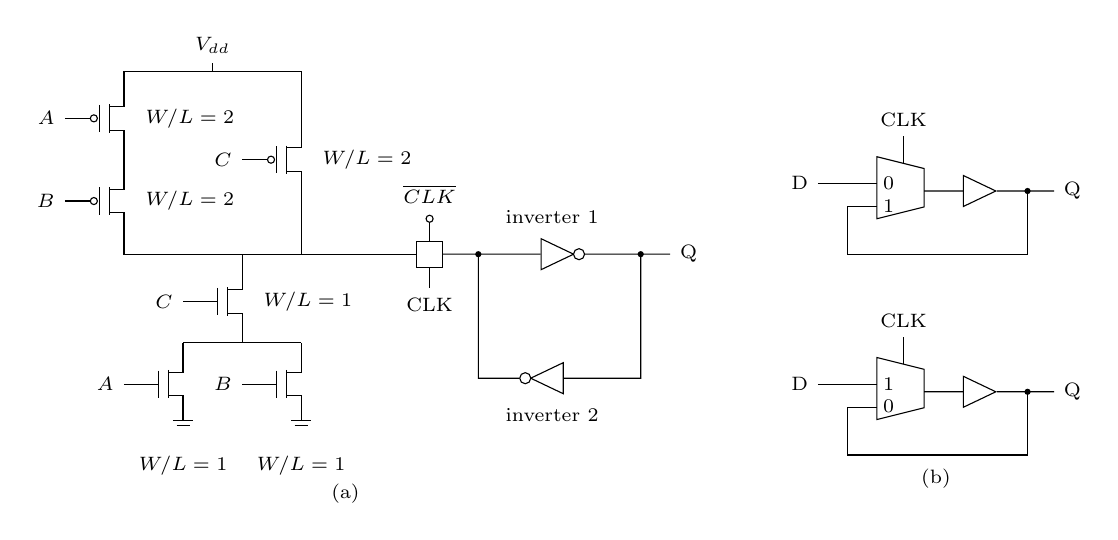
\begin{tikzpicture}[scale=.75,font=\scriptsize]
\mos{-2}{4.9}{A}{1}\mos{-2}{3.5}{B}{1}\mos{1}{4.2}{C}{1}\mos{0}{1.8}{C}{0}\mos{-1}{.4}{A}{0}\mos{1}{.4}{B}{0}
\draw(-1.75,5.4)--(-1.75,5.7)--(1.25,5.7)--(1.25,4.7);\rail{-.25}{5.7}{V_{dd}}\draw(-1.75,4.4)--(-1.75,4);\draw(-1.75,3)--(-1.75,2.6)--(1.25,2.6)--(1.25,3.7);\draw(.25,2.6)--(.25,2.3);\draw(.25,1.3)--(.25,1.1);\draw(-.75,1.1)--(1.25,1.1);\draw(-.75,1.1)--(-.75,.9);\draw(1.25,1.1)--(1.25,.9);\gnd{-.75}{-.1}\gnd{1.25}{-.1}
\foreach \x/\y in {-2/4.9,-2/3.5,1/4.2}{\node[right]at(\x+.45,\y){$W/L=2$};}\node[right]at(.45,1.8){$W/L=1$};\node[below]at(-.75,-.65){$W/L=1$};\node[below]at(1.25,-.65){$W/L=1$};
\draw(.25,2.6)--(3.2,2.6);\draw(3.2,2.38)rectangle(3.65,2.82);\draw(3.425,2.82)--(3.425,3.14);\draw(3.425,3.2)circle(.06);\node[above]at(3.425,3.3){$\overline{CLK}$};\draw(3.425,2.38)--(3.425,2.02)node[below]{CLK};
\node[not gate US,draw](i1)at(5.5,2.6){};\node[above]at(5.5,2.95){inverter 1};\draw(3.65,2.6)--(i1.input);\draw(i1.output)--(7.5,2.6)node[right]{Q};\fill(7,2.6)circle(1.5pt);
\node[not gate US,draw,rotate=180](i2)at(5.5,.5){};\node[below]at(5.5,.15){inverter 2};\draw(i2.input)--(7,.5)--(7,2.6);\draw(i2.output)--(4.25,.5)--(4.25,2.6);\fill(4.25,2.6)circle(1.5pt);\node at(2,-1.45){(a)};
\begin{scope}[xshift=10cm]
\foreach \y/\a/\b in {3.8/0/1,.4/1/0}{
\draw(0,\y)--(1,\y)node[pos=0,left]{D};\draw(1,\y+.45)--(1,\y-.6)--(1.8,\y-.4)--(1.8,\y+.25)--cycle;\node at(1.2,\y){$\a$};\node at(1.2,\y-.38){$\b$};\draw(1.45,\y+.34)--(1.45,\y+.8)node[above]{CLK};\node[buffer gate US,draw](buf\a)at(2.65,\y-.13){};\draw(1.8,\y-.13)--(buf\a.input);\draw(buf\a.output)--(4,\y-.13)node[right]{Q};\draw(3.55,\y-.13)--(3.55,\y-1.2)--(.5,\y-1.2)--(.5,\y-.4)--(1,\y-.4);\fill(3.55,\y-.13)circle(1.5pt);}
\node at(2,-1.2){(b)};\end{scope}
\end{tikzpicture}\\Figure 6: (a) Positive-active latch. (b) The two printed complementary-level latch drawings. The original caption/text also refer to panel (c), which is a panel-label typo; no third drawing is present.\end{center}\end{document}